%==========================================================================================================
% MULAI BAB IV
%==========================================================================================================
\chapter{PENGUJIAN DAN ANALISA}
\label{chap:pengujian}
%==========================================================================================================
% Subbab
%==========================================================================================================
Dalam pengujian aplikasi ini, ada dua cara pengujian yaitu dengan PC notebook yang dilengkapi \textit{webcam} internal atau menggunakan PC \textit{Desktop} dengan tambahan \textit{webcam}, konfigurasi sistem dapat dilihat pada gambar \ref{fig:monas_ar}. Untuk menjalankan aplikasi ini, diperlukan \textit{web browser} yang sudah terintegrasi \textit{plug-in} flash player versi 10. 

Spesifikasi sistem yang penulis gunakan dalam pengujian ini adalah sebagai berikut.
\begin{itemize}
\item Prosesor AMD Phenom\texttrademark II X4 955 Processor 3200 Mhz
\item Memori 2 Gb
\item standar usb 2.0 \textit{webcam} 
\item \textit{web browser} Mozilla Firefox versi 3.6.12
\end{itemize}

\begin{figure}[h]
\begin{center}
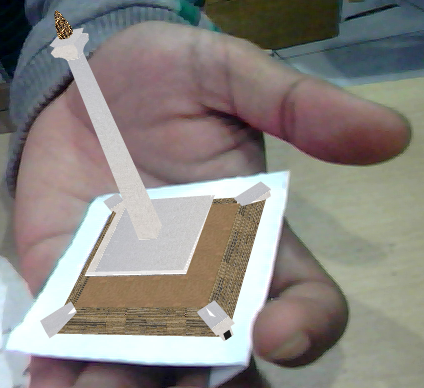
\includegraphics[width=6cm]{./images/ar3dv/monas_ar}
\caption{\label{fig:monas_ar} Hasil pengujian}
\end{center}
\end{figure}

Hasil pengujian dapat dilihat pada gambar \ref{fig:monas_ar}. Objek 3D dapat dirender dengan baik, meskipun kadang-kadang hilang dari marker, dikarenakan sistem tidak dapat menerima input dengan pergerakan yang marker cepat. Ada dua hal yang akan dianalisa yaitu fps (frame per second) dari video hasil rendering objek 3D dengan model yang berbeda-beda serta juga jarak dan sudut kemiringan marker yang masih dapat diterima aplikasi.

\section{Analisa \textit{Frame per Second (FPS)}}
\label{sec:analisa_fps}
\textit{Frame rate} atau frekuensi \textit{frame} merupakan frekuensi sebuah alat atau layar menghasilkan gambar yang disebut \textit{frame}. \textit{Frame rate} lebih sering dikenal dan diekspresikan sebagai frame per second (FPS). FPS merupakan jumlah gambar yang dihasilkan dalam waktu satu detik, mata manusia memerlukan jumlah \textit{frame} tertentu dalam satu detik agar dapat melihat gambar bergerak tanpa adanya \textit{flicker}. Jumlah FPS juga tergantung dari intensitas cahaya dan kecepatan objek bergerak dari video yang dihasilkan.

Pengujian untuk menganalisa FPS sangat diperlukan untuk mengetahui sejauh mana performa aplikasi viewer objek 3D ini. Untuk keperluan tersebut, penulis menambahkan informasi FPS tersebut ke aplikasi agar dapat dianalisa. Papervision3D telah menyediakan kelas untuk hal tersebut yaitu \textbf{StatsView}. Penggunaannya dapat dilihat dari \textit{listing} \ref{code:stats-view}.

\begin{lstlisting}[language=ActionScript,caption=StatsView,label=code:stats-view]
	_renderEngine = new LazyRenderEngine(_scene3D, _camera3D, _viewport3D);
	addChild(new StatsView(_renderEngine));
\end{lstlisting}

Sebuah informasi teks akan ditampilkan dikiri atas tampilan video, seperti yang ditunjukkan oleh gambar \ref{fig:fps_ar3dv}. Penulis menggunakan lima macam objek 3D berbeda dalam melakukan pengujian ini. Hasil pengujian dapat dilihat pada tabel \ref{tab:tabel_pengujian_fps}.

\begin{figure}[h]
\begin{center}
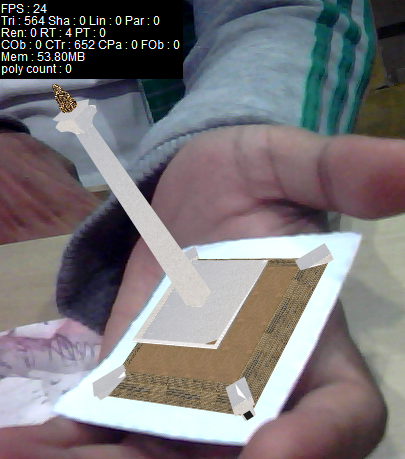
\includegraphics[width=6cm]{./images/ar3dv/monas_stats}
\caption{\label{fig:monas_stats} Hasil pengujian dengan statistik}
\end{center}
\end{figure}

\begin{table}[h]
\begin{center}
	\caption{Hasil Pengujian dengan Lima Model 3D}\label{tab:tabel_pengujian_fps}
	\vspace{5mm}
    \begin{tabular}[caption]{ | l | l | l | l | l | l | l |}
    \hline
    No & Nama & Tipe file & Ukuran file (KB) & FPS & Memory (MB) & Tri \cr \hline
    1 & airport & 3DS &  129,7 & 14 & 51,76 & 2870 \cr \hline
    2 & eiffel & DAE & 38,7 & 50 & 44,93 & 206 \cr \hline
	3 & monas & DAE & 154,5 & 24 & 53.80 & 564 \cr \hline
	4 & scout & DAE & 267,2 & 38 & 55.28 & 233 \cr \hline
	5 & tajmahal & DAE & 812,9 & 0 & 567.68 & 147.018 \cr \hline
    \hline
    \end{tabular}
\end{center}
\end{table}

Nilai FPS bergantung pada kompleksitas objek 3D yang ditampilkan. Untuk objek 3D yang tidak terlalu kompleks, hasilnya sangat baik, FPS berkisar antara 24 sampai 50, sehingga masih dapat terlihat baik. pada objek 3D kelima, nilai FPS nol atau tidak bergerak sama sekali, walaupun objek tersebut dapat terlihat. Penulis beranggapan bahwa frame yang dihasilkan dalam beberapa detik sekali, sehingga nilai FPS yang didapat adalah nol, hal ini disebabkan karena objek 3D yang di-\textit{render} sangat kompleks sehingga aplikasi tidak sanggup untum menampilkannya dengan baik.

%\section{Analisa Penggunaan Marker}
%\label{sec:analisa_marker}
%
%\subsection{Jarak}
%\label{subsec:analisa_jarak_marker}
%
%
%\subsection{Sudut Kemiringan}
%\label{subsec:analisa_sudut_marker}